\documentclass[11pt]{article}

\usepackage[margin=1in]{geometry}
\usepackage{booktabs}
\usepackage{microtype}
\usepackage{amsmath}
\usepackage{amssymb}
\usepackage{bm}
\usepackage{enumitem}
\usepackage{graphicx}
\usepackage{caption}
\usepackage{subcaption}
\usepackage{xcolor}
\usepackage{colortbl}
\usepackage{array}
\usepackage{algorithm}
\usepackage{algpseudocode}
\usepackage[hidelinks]{hyperref}

\definecolor{linkblue}{HTML}{2A5DB0}
\definecolor{teal}{HTML}{0F7F7B}
\definecolor{rowhi}{HTML}{EAF4F0}

\hypersetup{
  colorlinks=true, linkcolor=linkblue, citecolor=linkblue, urlcolor=teal,
  pdftitle={TokenTriage: Harm-Aware Token Routing for Clinical Language Model Inference},
  pdfauthor={Kelly Powell, Danish Murad, Benjamin A. Willett, Richard Carlisle, Bryan Webb, Sandeep Bodduluri}
}

\captionsetup{font=small,labelfont=bf,labelsep=period}
\captionsetup[sub]{font=small,labelfont=bf}

\newcommand{\method}{\mbox{TokenTriage}}
\newcommand{\repoURL}{\url{https://github.com/DIGlabUAB/token-triage}}
\newcommand{\critset}{\mathcal{C}}
\newcommand{\argmax}{\operatornamewithlimits{arg\,max}}

\usepackage{titlesec}
\titlespacing*{\section}{0pt}{1.6ex plus 1ex minus .2ex}{1.0ex plus .2ex}
\titlespacing*{\subsection}{0pt}{1.2ex plus .8ex minus .2ex}{0.6ex plus .2ex}

\title{\vspace{-1.2em}\textbf{\method{}: Harm-Aware Token Routing for\\Clinical Language Model Inference}}
\author{%
  Kelly Powell, MBA \quad Danish Murad, M.S. \quad Benjamin A. Willett, Ph.D.\\[2pt]
  Richard Carlisle, B.S., CISSP \quad Bryan Webb, B.S. \quad Sandeep Bodduluri, M.S., Ph.D.\\[4pt]
  \small\href{mailto:sbodduluri@uabmc.edu}{sbodduluri@uabmc.edu} (corresponding author)
}
\date{June 2026}

\begin{document}
\maketitle
\vspace{-0.8em}

\begin{figure}[h!]
  \centering
  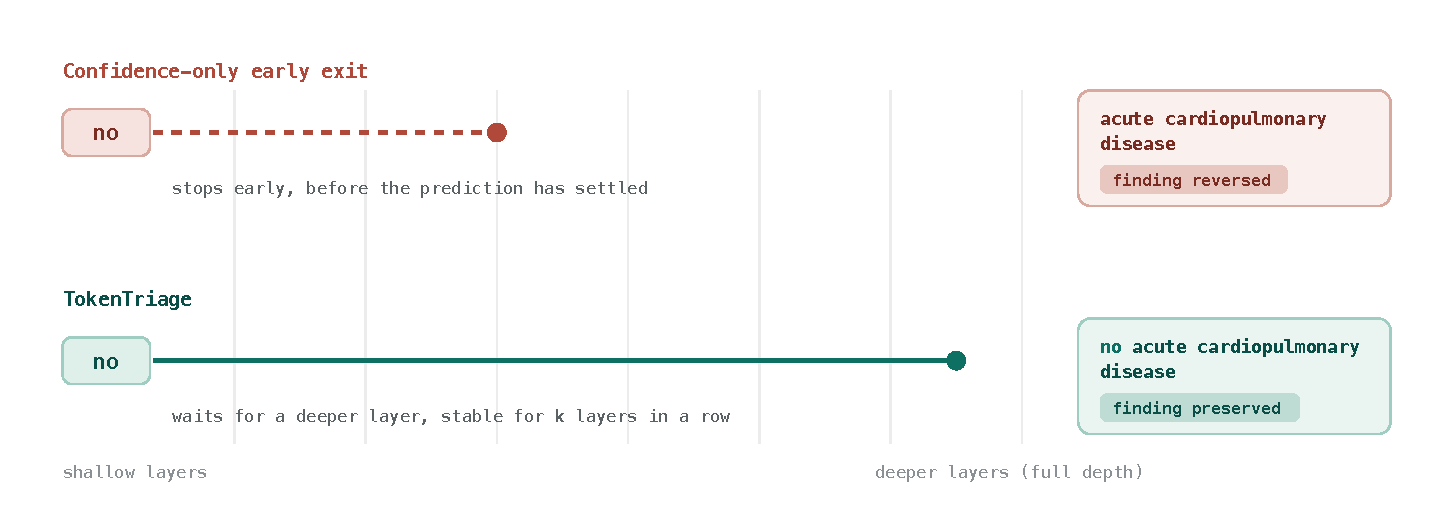
\includegraphics[width=\linewidth]{figures/overview.pdf}
  \caption{Overview of \method{}. The clinically critical word \emph{no} is decoded two ways by the
  same model. A confidence-only early exit stops at a shallow layer, before the prediction has settled,
  and drops the negation, so the report reads \emph{acute cardiopulmonary disease} and the finding is
  reversed. \method{} holds the same word until a deeper layer at which the top prediction has been
  stable for $k$ consecutive layers, which preserves \emph{no} and the original finding. Ordinary words
  still take the cheap early exit, so most of the compute saving is kept.}
  \label{fig:overview}
\end{figure}

\vspace{-0.4em}
\begin{abstract}
\noindent
Adaptive-inference methods such as early exit reduce language-model compute by stopping computation
at an intermediate layer when the prediction for a token already looks confident. We argue that for clinical
text, an average compute-quality trade-off is the wrong thing to optimize, because clinical language
is semantically asymmetric. An early error on \emph{no}, \emph{left}, \emph{severe}, a measurement, or
a disease term can invert the meaning of a report, while an early error on a function word is
harmless. We formalize a harm-stratified view of adaptive inference and measure preservation of the
full model at the token level, conditioned on clinical semantic risk. Across four open models
(Qwen2.5-0.5B/1.5B/3B and SmolLM2-1.7B; two architecture families and a 6x parameter range) and two
public radiology datasets, the strongest confidence-only early exit, at a compute saving of 37.9\%,
disagrees with the full model on 71.7\% of clinically critical tokens on 256 IU~X-Ray reports. We
introduce \method{}, a routing rule that leaves ordinary tokens to a confidence exit but requires
critical tokens to reach a minimum depth and $k$ consecutive stable predictions. It reduces
critical-token disagreement to 24.9\% (95\% CI $[0.226,0.276]$) at comparable savings. We validate the
effect against ground truth in two ways. Measured against the exact words of the radiologist, confidence-only
exit introduces 16 to 22 points of excess critical-token error over the full model, while \method{}
introduces 0 to 4. A CheXbert counterfactual shows that \method{} roughly halves both the reports whose
clinical findings change (70\% down to 46\%) and the total findings flipped (400 down to 224). Finally,
we report a negative result that places the contribution honestly: untrained free-running early-exit
generation collapses for all policies, so \method{} belongs in the preservation and verification
regime, most directly as harm-aware acceptance for self-speculative decoding, rather than as a
standalone generation speedup. Code, traces, and analyses are released openly.
\end{abstract}

\section{Introduction}
\label{sec:intro}
A transformer language model spends the same computation on every token, regardless of how much that
token matters. Adaptive-computation methods use the observation that many tokens are easy, in the
sense that their final prediction is already settled at an intermediate layer, and stop early to save
latency and cost \cite{branchynet,deebert,fastbert,calm,layerskip}. The usual exit criteria are local
measures of model confidence: the entropy of the intermediate distribution, the top-1 minus top-2
margin, or the response of a trained early-exit classifier.

Confidence is a property of the model, not of the cost of being wrong. In clinical documentation the
two come apart. Consider the phrase ``\emph{no} acute pulmonary edema.'' The token \emph{no} may be
low or high entropy at a given layer, but its semantic leverage is large: an early commitment to the
wrong token here reverses the finding. The same holds for laterality (\emph{left} or \emph{right}),
severity (\emph{mild} or \emph{severe}), temporality (\emph{new} or \emph{chronic}), numeric
measurements, and named findings. A function word like \emph{the} carries no such leverage. An
efficiency method that allocates compute by confidence alone is therefore blind to the dimension that
matters clinically.

This paper asks a narrow question. When adaptive inference saves compute on clinical text, is the
saving drawn disproportionately from the tokens whose errors carry clinical risk? We answer it by
measuring preservation of the full-model prediction at the token level, stratified by a semantic
risk label, and, because preservation is not the same as correctness, also against the gold
radiologist text and against a clinical entity labeler. We then propose a small intervention that
reallocates compute by risk rather than by confidence alone.

\paragraph{Scope: where adaptive depth fits.}
We want to be clear about deployment relevance. Post-training quantization \cite{llmint8,gptq,awq} and
distillation are the dominant techniques in use today for fast LLM inference, and they reduce cost on a
different axis (numerical precision and model size) than adaptive depth. Early exit is complementary
to both, since a quantized model can still exit early, and its most widely used relative is
self-speculative decoding, in which early-exit drafts are verified by the full model \cite{layerskip}.
We do not claim that adaptive depth should replace quantization. The contribution is a harm-aware lens,
and a routing or verification rule, for the adaptive-depth family when it is applied to clinical text,
where the question of which drafts to trust without a full-model check is itself a semantic-risk
decision.

\paragraph{Contributions.}
\begin{enumerate}[leftmargin=1.5em,itemsep=2pt,topsep=2pt]
  \item A harm-stratified evaluation of adaptive inference (Section~\ref{sec:formulation}): an objective
        that conditions preservation of the full model on clinical semantic risk, which exposes a
        failure mode that average compute-quality curves hide.
  \item \method{} (Section~\ref{sec:method}, Algorithm~\ref{alg:tt}): a simple, training-free routing
        rule that combines a confidence exit for ordinary tokens with a depth and $k$-stability
        requirement for critical tokens, together with a pluggable risk-tagger interface.
  \item Evidence across models, datasets, and ground truth (Section~\ref{sec:results}): confidence-only
        adaptive inference concentrates error on critical tokens across two model families and a 6x size
        range, on a second dataset, against the exact words of the radiologist, and, through a CheXbert
        counterfactual, at the level of clinical findings.
  \item An honest decoding-regime analysis (Section~\ref{sec:decoding}): untrained free-running
        early-exit generation collapses regardless of policy, which places the contribution in the
        preservation and verification regime and connects it to self-speculative decoding.
\end{enumerate}

\section{Related Work}
\label{sec:related}

\paragraph{Efficient inference.}
The dominant production techniques reduce precision or size: post-training quantization to 8-bit
\cite{llmint8} and to 3 or 4 bits \cite{gptq,awq}, knowledge distillation \cite{distillation2015,distilbert2019},
and one-shot pruning \cite{sparsegpt2023}. These act on a different axis from the depth axis studied
here and compose with it, which is why we treat adaptive depth as complementary rather than competing.

\paragraph{Adaptive computation and early exit.}
Adaptive computation time learned to spend a variable number of steps per token \cite{graves2016}, and
PonderNet reframed this as a learned halting distribution \cite{pondernet2021}. For transformers
\cite{vaswani2017}, BranchyNet attached side classifiers so confident inputs could exit early
\cite{branchynet}, the depth-adaptive transformer learned per-token exit depths \cite{depthadaptive2020},
and DeeBERT, FastBERT, PABEE, and the right-tool-for-the-job line brought input-adaptive exiting to
encoders by confidence or patience \cite{deebert,fastbert,pabee2020,righttool2020}. CALM extended
adaptive computation to autoregressive generation with calibrated local confidence measures and a
consistency guarantee \cite{calm}, while mixture-of-depths routes a compute budget across positions
\cite{mixtureofdepths2024}. LayerSkip trains a model with layer dropout and an early-exit loss so that
early exit and self-speculative decoding work without auxiliary heads \cite{layerskip}. All of these
select exits by confidence, calibration \cite{calibration2017}, or a trained acceptance criterion, and
none condition on the semantic consequence of the token, which is our focus.

\paragraph{Speculative and self-speculative decoding.}
Speculative decoding speeds up generation by drafting with a cheap model and verifying with the target
model \cite{speculative2023,specsampling2023}, and variants such as Medusa and EAGLE add lightweight
draft heads \cite{medusa2024,eagle2024}. Self-speculative decoding uses the early layers of the model
as the drafter \cite{layerskip}. This is the most realistic deployment path for adaptive depth, and it
is a setting where a harm-aware acceptance rule, one that trusts cheap drafts for ordinary tokens but
asks for full-model confirmation on critical ones, is natural.

\paragraph{Clinical report understanding.}
RadGraph extracts clinical entities and relations from radiology reports \cite{radgraph2021}, and
CheXbert \cite{chexbert} labels reports with the 14 standard CheXpert chest-radiograph findings
\cite{chexpert2019}. Both are used to evaluate clinical text generation. We use CheXbert to convert
token-level error into a clinical-finding-level measure of harm (Section~\ref{sec:entity}). To our
knowledge, prior efficiency work for clinical LLMs has not stratified adaptive-inference error by
semantic risk.

\section{Problem Formulation}
\label{sec:formulation}
Let a report be a token sequence $\bm{x} = (x_1,\dots,x_n)$ processed by an $L$-layer transformer. For
position $i$, let $\bm{h}_i^{(\ell)}$ be the hidden state after layer $\ell$. The logit lens, an
unembedding probe of intermediate states \cite{tunedlens2023}, projects a state to the vocabulary using
the final norm of the model $\mathrm{LN}$ and unembedding $W_U$:
\begin{equation}
\bm{z}_i^{(\ell)} = W_U\,\mathrm{LN}\!\big(\bm{h}_i^{(\ell)}\big),
\qquad
\bm{p}_i^{(\ell)} = \mathrm{softmax}\big(\bm{z}_i^{(\ell)}\big).
\end{equation}
Write the layer-$\ell$ prediction $\hat{y}_i^{(\ell)} = \argmax_v \bm{p}_i^{(\ell)}(v)$, and the
full-model prediction $\hat{y}_i^{(L)}$. An exit policy $\pi$ assigns each position an exit layer
$e_i = \pi(i) \in \{1,\dots,L\}$ and emits $\hat{y}_i^{(e_i)}$. Its simulated compute saving is
$1 - \tfrac{1}{nL}\sum_i e_i$.

\paragraph{Semantic risk.}
A risk tagger $c$, mapping each token to a value in $[0,1]$, assigns each position a criticality $c_i = c(x_i)$, and the
set of critical positions is $\critset = \{i : c_i \ge \tau_c\}$ with $\tau_c = 0.8$. We treat $c$ as a
pluggable interface (Section~\ref{sec:risk}).

\paragraph{Harm-stratified preservation.}
The quantity of interest is not average accuracy but where a policy deviates from the full model. We
define critical-token disagreement
\begin{equation}
\mathrm{D}_\critset(\pi) \;=\; \frac{1}{|\critset|}\sum_{i\in\critset}
\mathbb{1}\!\left[\hat{y}_i^{(e_i)} \neq \hat{y}_i^{(L)}\right],
\end{equation}
and harm-weighted disagreement $\mathrm{HWD}(\pi)=\big(\sum_i c_i \,\mathbb{1}[\hat
y_i^{(e_i)}\neq\hat y_i^{(L)}]\big)/\sum_i c_i$. A good clinical policy minimizes $\mathrm{D}_\critset$
at a given compute saving, even at the cost of higher disagreement on ordinary tokens.

\section{Method}
\label{sec:method}

\subsection{Layerwise tracing}
We run each report teacher-forced once and cache, for every $(i,\ell)$, the normalized entropy, the
top-1 minus top-2 margin, the target negative log-likelihood, the top token $\hat y_i^{(\ell)}$, and the
agreement indicator $\mathbb{1}[\hat y_i^{(\ell)}=\hat y_i^{(L)}]$:
\begin{equation}
H_i^{(\ell)} = \frac{-1}{\log |V|}\sum_v \bm{p}_i^{(\ell)}(v)\log \bm{p}_i^{(\ell)}(v),
\qquad
M_i^{(\ell)} = \bm{p}_i^{(\ell)}{\scriptstyle(1)} - \bm{p}_i^{(\ell)}{\scriptstyle(2)} .
\end{equation}
Caching separates tracing from policy evaluation, so every policy below is scored on identical traces,
which makes the comparisons exact and cheap.

\subsection{Risk assignment (pluggable)}
\label{sec:risk}
The default tagger is a clinical lexicon that flags negation, laterality, severity, temporality,
medication, numeric measurement, measurement unit, and key findings (for example \texttt{no},
\texttt{left}, \texttt{severe}, \texttt{2.4}, \texttt{cm}, \texttt{effusion}). The tagger is an
interface: any function that maps a token to a value in $[0,1]$, including a RadGraph- or
CheXbert-derived tagger, can be registered without modifying the routing or evaluation code.

\subsection{Policies}
We evaluate four reference policies and \method{}. The entropy exit stops at the first layer with
$H_i^{(\ell)}\le\tau$, the margin exit at the first with $M_i^{(\ell)}\ge\gamma$, fixed-depth at
$\lceil\rho L\rceil$, and a non-causal stability oracle at the first layer after which
$\hat y_i^{(\ell)}=\hat y_i^{(L)}$ for all deeper layers, which is an upper bound on achievable
preservation.

\subsection{TokenTriage}
\method{} (Algorithm~\ref{alg:tt}) applies the entropy exit to ordinary tokens but holds critical
tokens to two extra requirements: a minimum depth $\lceil\rho L\rceil$, and $k$-stability, meaning the
top prediction must be unchanged for $k$ consecutive layers. The second requirement is evidence that
the early decision is not an artifact of an unsettled intermediate representation. Unless stated
otherwise we use $\tau=0.10$, $\rho=0.85$, and $k=4$.

\begin{algorithm}[t]
\caption{\method{} exit decision for position $i$}
\label{alg:tt}
\begin{algorithmic}[1]
\Require per-layer top tokens $\hat y_i^{(1:L)}$, entropies $H_i^{(1:L)}$, criticality $c_i$;
threshold $\tau$, min.\ fraction $\rho$, patience $k$
\State $b \gets \min\{\ell : H_i^{(\ell)} \le \tau\}$ \quad(set $b\gets L$ if none) \Comment{confidence exit}
\If{$c_i < \tau_c$} \State \Return $b$ \Comment{ordinary token: cheap exit}
\EndIf
\State $\ell_{\min} \gets \lceil \rho L \rceil$
\For{$\ell = \max(b,\,\ell_{\min},\,k)$ \textbf{to} $L$}
  \If{$\hat y_i^{(\ell-k+1)} = \cdots = \hat y_i^{(\ell)}$} \State \Return $\ell$ \Comment{$k$-stable}
  \EndIf
\EndFor
\State \Return $L$
\end{algorithmic}
\end{algorithm}

\subsection{Correctness and entity-level metrics}
Beyond preservation we report two ground-truth metrics. Let $g_i$ be the gold (radiologist) token. The
excess critical-token error is the extra error a policy makes over the full model,
$\Delta(\pi)=\frac{1}{|\critset|}\sum_{i\in\critset}\big(\mathbb{1}[\hat y_i^{(e_i)}\neq
g_i]-\mathbb{1}[\hat y_i^{(L)}\neq g_i]\big)$, which removes the high intrinsic floor of exact
next-token prediction. The entity-level harm metric (Section~\ref{sec:entity}) replaces each critical
position in the gold report with the prediction of the policy and labels the gold and perturbed reports with
CheXbert, counting changes to the 14-dimensional finding vector.

\section{Experimental Setup}
\label{sec:setup}
\paragraph{Data and models.}
The primary experiment uses the public \texttt{ChayanM/IUXray-Data-Train-Test} test split (256 reports,
13{,}697 next-token positions, 1{,}163 critical tokens, $L{=}28$) with Qwen2.5-1.5B-Instruct
\cite{qwen25}. We test generalization on Qwen2.5-0.5B/1.5B/3B ($L=24/28/36$) and SmolLM2-1.7B
\cite{smollm2} ($L=24$) at 64 reports, and on a
second dataset, \texttt{Santhosh1705kumar/radiology-reports-chest} (ROCO chest captions, 64 reports).
All data and models are public.

\paragraph{Protocol.}
Hidden states are computed in \texttt{float16} on Apple MPS. Confidence intervals are report-level
bootstraps (200 resamples), resampling reports to respect within-report correlation. The compute saving
is the simulated layer fraction $1-\bar{e}/L$. We sweep $\tau\in\{0.10,\dots,0.55\}$ and
$\gamma\in\{0.05,\dots,0.50\}$ and report the strongest confidence baseline by $\mathrm{D}_\critset$.

\section{Results}
\label{sec:results}

\subsection{Confidence-only exit concentrates error on critical tokens}
\begin{table}[h]
\centering\small
\setlength{\tabcolsep}{6pt}\renewcommand{\arraystretch}{1.15}
\begin{tabular}{llrrcr}
\toprule
Method & Setting & Compute saved & $\mathrm{D}_\critset$ & 95\% CI & HWD \\
\midrule
Entropy & $\tau{=}0.10$ & 0.379 & 0.717 & [0.686,0.747] & 0.560 \\
Margin & $\gamma{=}0.50$ & 0.571 & 0.865 & [0.848,0.884] & 0.779 \\
\rowcolor{rowhi}
\method{} & $\tau{=}0.10,\rho{=}0.85,k{=}4$ & 0.331 & \textbf{0.249} & [0.226,0.276] & 0.390 \\
\method{} & $\tau{=}0.20,\rho{=}0.85,k{=}4$ & 0.517 & 0.270 & [0.247,0.297] & 0.575 \\
\bottomrule
\end{tabular}
\caption{Main result on 256 IU~X-Ray reports with Qwen2.5-1.5B. Confidence-only exits save compute but
concentrate disagreement on critical tokens. \method{} more than halves it at comparable savings, and
the result is stable versus the 64-report run (0.721 down to 0.255).}
\label{tab:main}
\end{table}

The strongest confidence baseline (entropy, $\tau{=}0.10$) saves 37.9\% of simulated compute yet
disagrees with the full model on 71.7\% of critical tokens (Table~\ref{tab:main}). \method{} at the
matched threshold reduces $\mathrm{D}_\critset$ to 24.9\%, a 46.9 point absolute reduction, while
retaining 33.1\% savings, and the bootstrap intervals do not overlap. A higher-savings operating point
($\tau{=}0.20$) reaches 51.7\% savings at 27.0\%, still well below the baseline.

\begin{figure}[h]
  \centering
  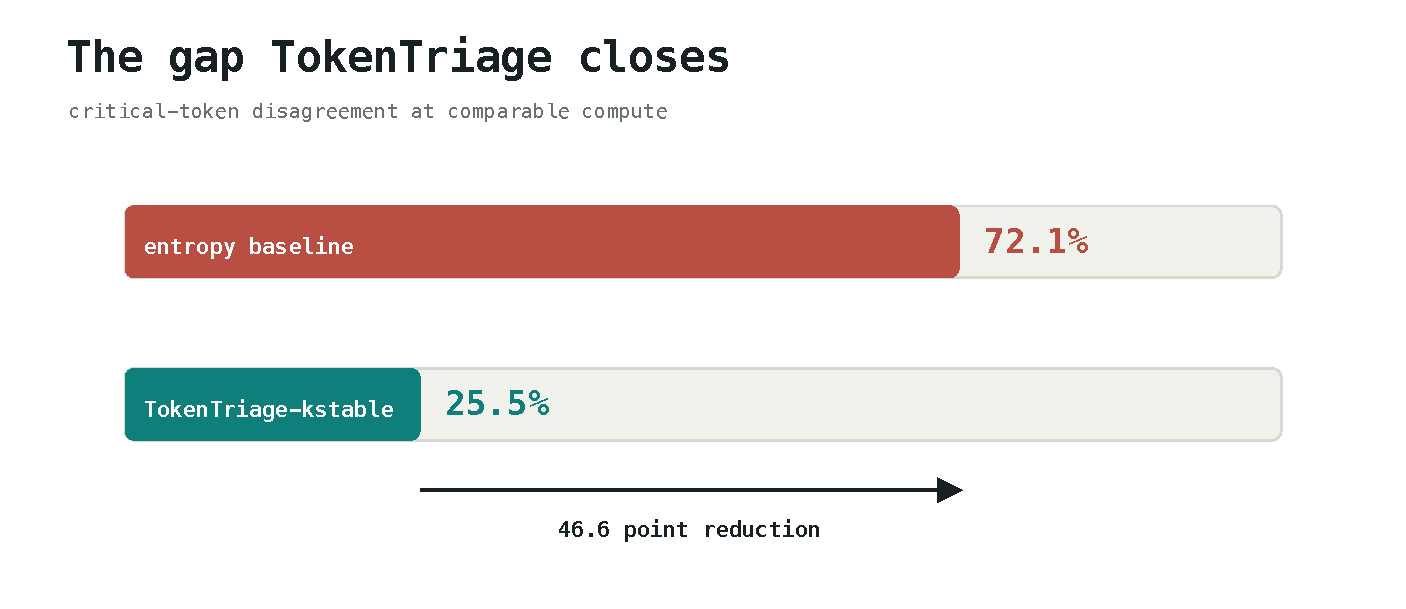
\includegraphics[width=0.82\linewidth]{figures/gap.pdf}
  \caption{The same comparison on the 64-report sample. At comparable compute savings, the
  confidence-only entropy exit disagrees with the full model on the majority of critical tokens, while
  \method{} closes most of the gap. The model and the traces are identical; only the halting rule for
  high-risk tokens differs.}
  \label{fig:gap}
\end{figure}

\subsection{Generalization across families, scale, and dataset}
\begin{figure}[h]
  \centering
  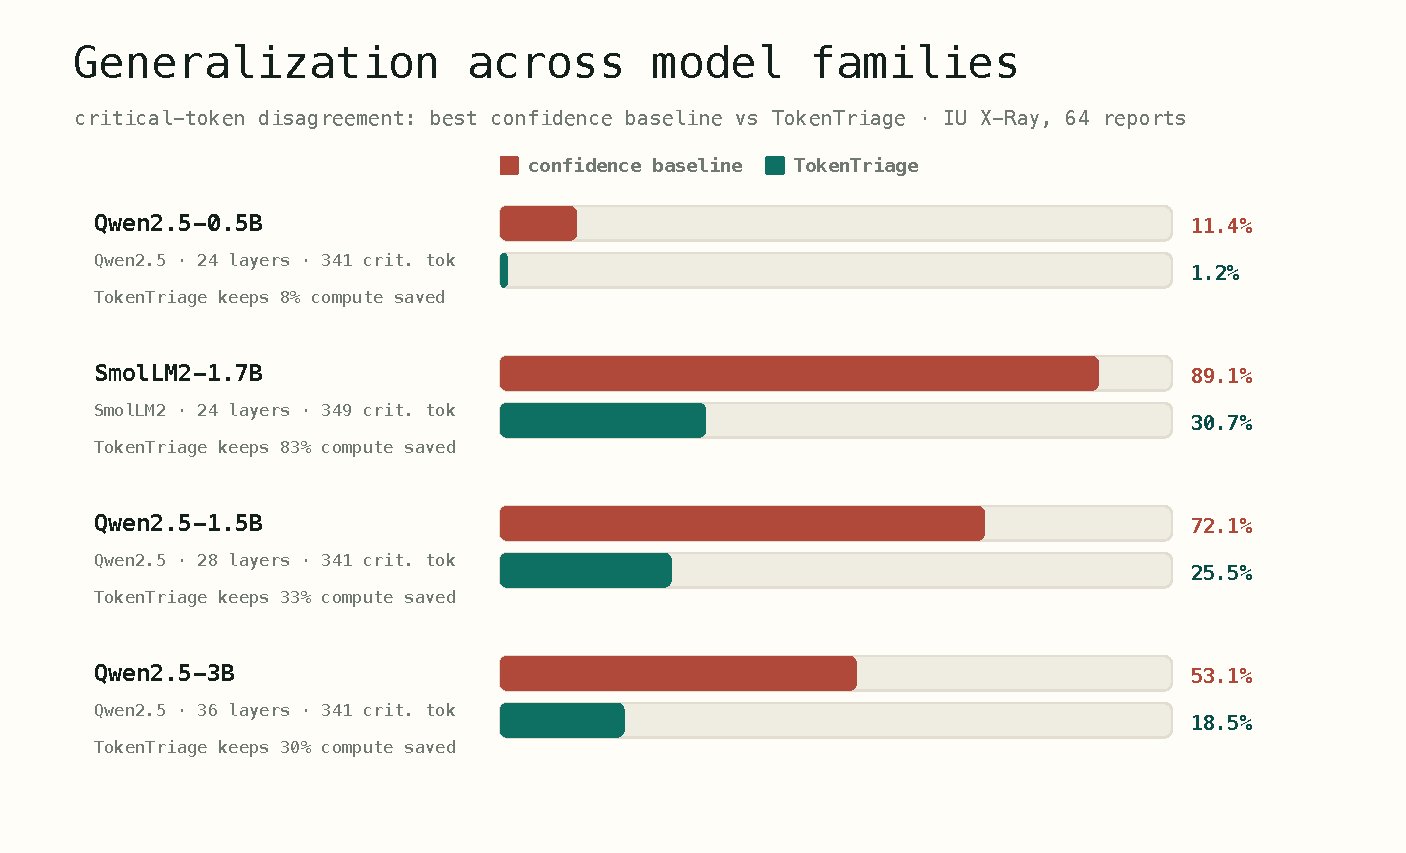
\includegraphics[width=0.95\linewidth]{figures/models.pdf}
  \caption{Critical-token disagreement across four open models (two families, 0.5B to 3B) on the same
  IU~X-Ray reports. \method{} (teal) is well below the confidence baseline (clay) in every case. Smaller
  models show a smaller gap, because when the baseline is already safe there is little to fix.}
  \label{fig:models}
\end{figure}

\begin{table}[h]
\centering\small
\setlength{\tabcolsep}{6pt}\renewcommand{\arraystretch}{1.12}
\begin{tabular}{llrrrr}
\toprule
Model / setting & Family & $|\critset|$ & Baseline $\mathrm{D}_\critset$ & \method{} & Saved \\
\midrule
Qwen2.5-0.5B (64) & Qwen2.5 & 341 & 0.114 & \textbf{0.012} & 0.085 \\
Qwen2.5-1.5B (64) & Qwen2.5 & 341 & 0.721 & \textbf{0.255} & 0.329 \\
Qwen2.5-3B (64) & Qwen2.5 & 341 & 0.531 & \textbf{0.185} & 0.297 \\
SmolLM2-1.7B (64) & SmolLM2 & 349 & 0.891 & \textbf{0.307} & 0.830 \\
\midrule
Qwen2.5-1.5B (256) & Qwen2.5 & 1163 & 0.717 & \textbf{0.249} & 0.331 \\
ROCO / Qwen2.5-1.5B (64) & Qwen2.5 & 150 & 0.620 & \textbf{0.153} & 0.273 \\
\bottomrule
\end{tabular}
\caption{Generalization (top), plus scale and a second dataset (bottom). The pattern is consistent, and
the 256-report run confirms it is not a small-sample artifact.}
\label{tab:generalize}
\end{table}

\subsection{Correctness against the words of the radiologist}
Because the teacher-forced text is the gold report, exact next-token match is a ground-truth signal.
Its floor is high, since free prose admits synonyms, so we report the excess $\Delta(\pi)$ rather than
the raw rate. Table~\ref{tab:gold} and Figure~\ref{fig:correct} show that confidence-only exit adds 16 to
22 points of excess critical-token error against the words of the radiologist, while \method{} adds 0 to 4.

\begin{table}[h]
\centering\small
\setlength{\tabcolsep}{6pt}\renewcommand{\arraystretch}{1.12}
\begin{tabular}{lrrr}
\toprule
Model & Full-model floor & Entropy excess $\Delta$ & \method{} excess $\Delta$ \\
\midrule
Qwen2.5-0.5B & 0.771 & +0.021 & \textbf{+0.000} \\
Qwen2.5-1.5B & 0.757 & +0.167 & \textbf{+0.024} \\
Qwen2.5-3B & 0.733 & +0.173 & \textbf{+0.029} \\
SmolLM2-1.7B & 0.782 & +0.215 & \textbf{+0.020} \\
Qwen2.5-1.5B (256) & 0.742 & +0.190 & \textbf{+0.025} \\
ROCO / Qwen2.5-1.5B & 0.693 & +0.187 & \textbf{+0.040} \\
\bottomrule
\end{tabular}
\caption{Excess critical-token error against the gold report token, over the full model.}
\label{tab:gold}
\end{table}

\begin{figure}[h]
  \centering
  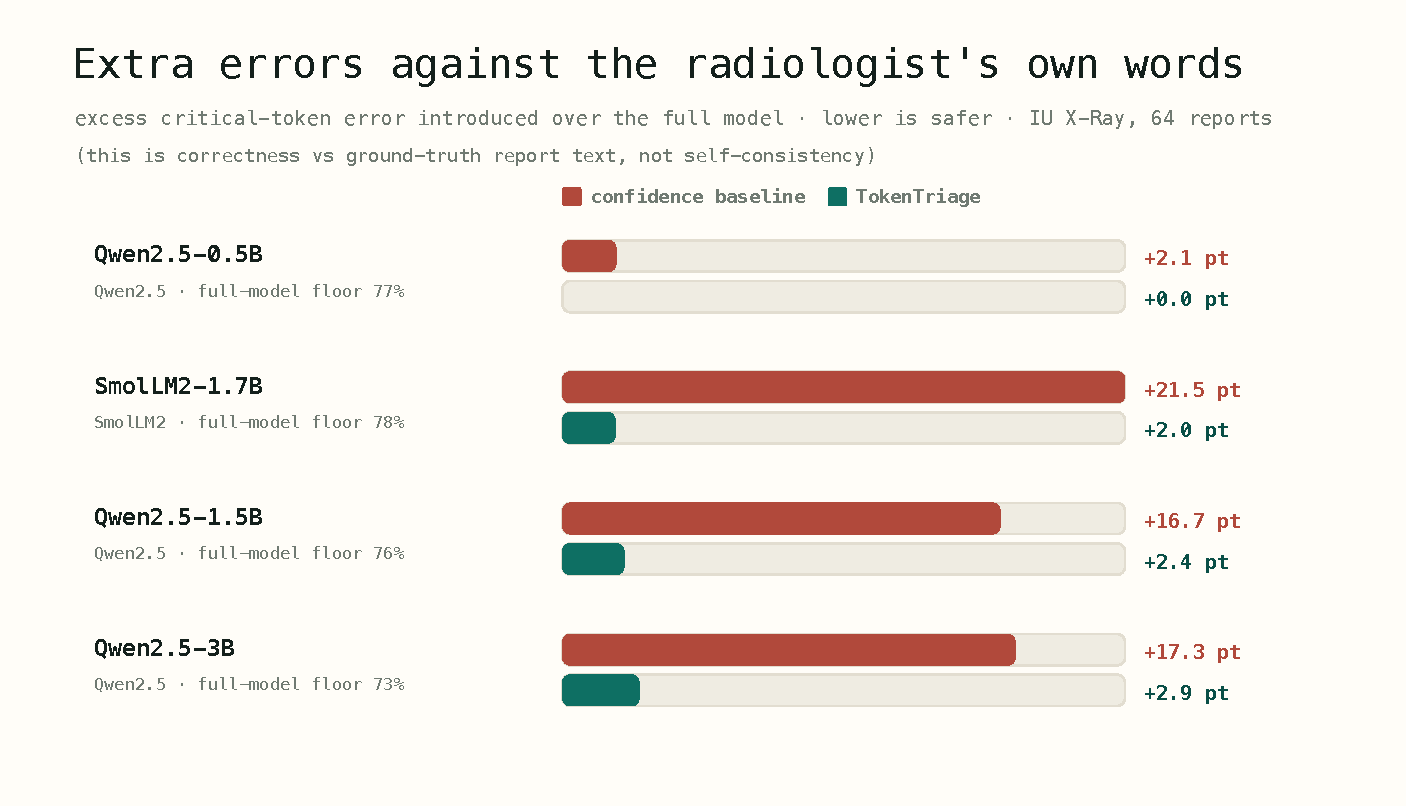
\includegraphics[width=0.9\linewidth]{figures/correctness.pdf}
  \caption{Excess critical-token error against the words of the radiologist. Confidence-only exit (clay) adds
  16 to 22 points, while \method{} (teal) adds 0 to 3.}
  \label{fig:correct}
\end{figure}

\subsection{Entity-level correctness with CheXbert}
\label{sec:entity}
Not every token error is clinically meaningful. We test the impact directly: we apply the critical-token errors of each policy to the gold report and label the gold and perturbed reports with CheXbert
\cite{chexbert}, then count changes to the finding vector. On the 256-report run, the critical-token
errors of confidence-only exit change at least one finding in 69.9\% of reports and flip 400
finding-labels overall. \method{} reduces this to 46.1\% and 224, a 44\% reduction
(Table~\ref{tab:entity}, Figure~\ref{fig:entity}). \method{} does not eliminate clinical change, which
is the honest residual, but it roughly halves it.

\begin{table}[h]
\centering\small
\setlength{\tabcolsep}{6pt}\renewcommand{\arraystretch}{1.15}
\begin{tabular}{lrrrr}
\toprule
& \multicolumn{2}{c}{Reports w/ changed finding} & \multicolumn{2}{c}{Findings flipped} \\
\cmidrule(lr){2-3}\cmidrule(lr){4-5}
Run & Entropy & \method{} & Entropy & \method{} \\
\midrule
IU X-Ray (256) & 0.699 & \textbf{0.461} & 400 & \textbf{224} \\
IU X-Ray (64) & 0.750 & \textbf{0.516} & 99 & \textbf{67} \\
\bottomrule
\end{tabular}
\caption{Entity-level correctness (CheXbert, Qwen2.5-1.5B). \method{} roughly halves clinical-finding
changes relative to confidence-only exit.}
\label{tab:entity}
\end{table}

\begin{figure}[h]
  \centering
  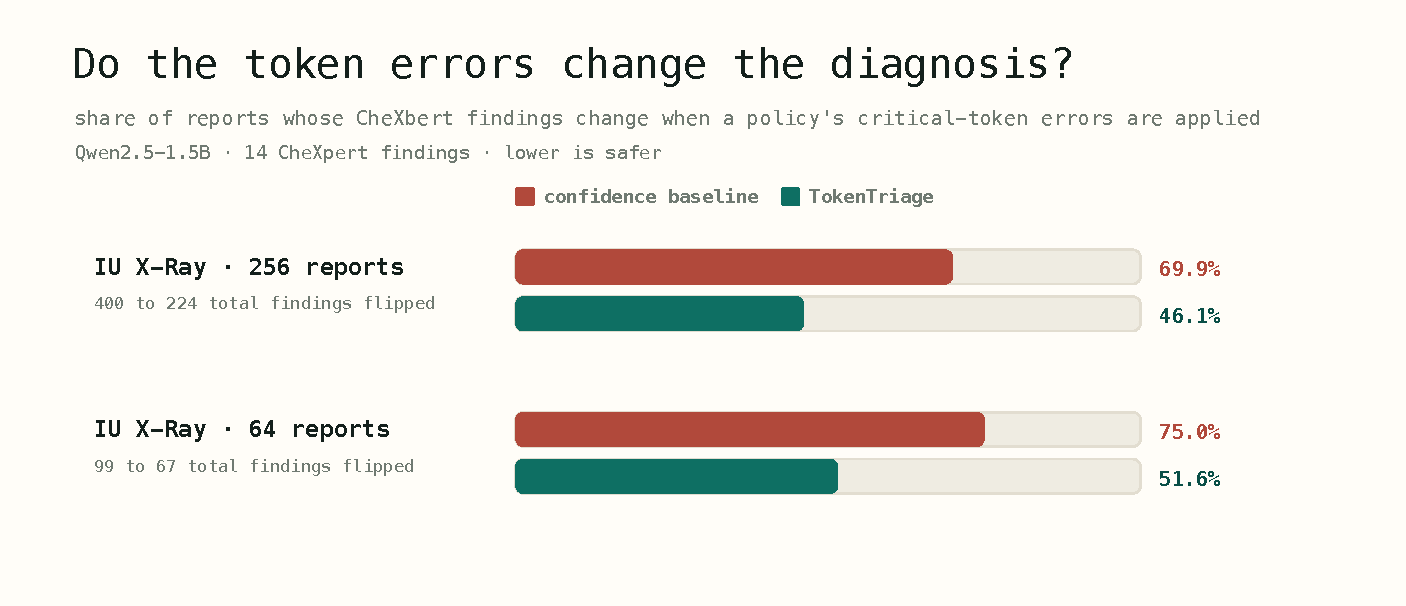
\includegraphics[width=0.86\linewidth]{figures/entity.pdf}
  \caption{Share of reports whose CheXbert findings change when the critical-token errors of a policy are
  applied to the gold report.}
  \label{fig:entity}
\end{figure}

\subsection{The decoding regime: an honest negative}
\label{sec:decoding}
The results above hold in the preservation regime, where the conditioning text is fixed (teacher
forcing, scoring, grounded generation, and speculative-decoding verification). We tested whether
harm-aware routing also helps during free, autoregressive generation by implementing real early-exit
decoding, in which each emitted token is chosen at its exit layer and fed back, so that errors
propagate. We compared full, entropy, and \method{} decoders on 24 IU~X-Ray continuations
(Qwen2.5-1.5B, $\tau{=}0.10$). The finding is negative. Untrained logit-lens early exit collapses for
both policies (prefix agreement with the full model near 2\%, critical-term fidelity near 0.10), and
\method{} changed the emitted token in 0 of 7 critical interventions. When a model freely generates a
critical token it is already confident, so the cheap-exit token is stable and harm-gating does not
fire. This is consistent with why deployed systems train exit heads \cite{calm,layerskip} rather than
read a raw logit lens, and it locates the value of \method{} where the target text is given, namely
verification and self-speculative-decoding acceptance, rather than in naive untrained generation.

\section{Discussion}
\label{sec:discussion}
Our results support a single claim: the compute-quality frontier is the wrong object for clinical
adaptive inference, because it averages over a semantically asymmetric token distribution. A policy can
look attractive in aggregate while concentrating both model-preservation error and ground-truth error
on the tokens that determine the meaning of the report. \method{} shows that a small, training-free
change to the halting rule, spending a few extra layers only on high-risk tokens, removes most of that
concentrated error, and the effect is consistent across two model families, a sixfold range of model
size, a second dataset, the words written by the radiologist, and the findings recovered by CheXbert.

We do not read this as an argument that adaptive depth should replace quantization. Quantization and
distillation reduce cost on the axis of numerical precision and model size, adaptive depth reduces it
on the axis of computation per token, and the two compose: a quantized model can still exit early. The
most realistic deployment for adaptive depth is therefore self-speculative decoding, where early-exit
drafts are accepted if they match the full model and otherwise corrected. Standard acceptance is
lossless but pays full-model compute on every token, whereas a harm-aware variant can accept cheap
drafts for ordinary tokens while requiring full-model confirmation only for critical ones, recovering
latency without the clinical risk that uniform aggressive acceptance would incur. The risk tagger and
stability criterion of \method{} are precisely the acceptance policy such a system needs, and our
preservation metric is precisely its acceptance rate.

These conclusions should be read with their limits in view, and we state them plainly. Preservation
and excess gold-token error are token-level proxies, and the CheXbert experiment measures changes to
the finding vector of a counterfactually perturbed gold report, not a radiologist judgment of report
correctness; a wrong token that does not move a CheXbert label may still matter clinically, and the
converse is possible as well. The logit lens we use to read intermediate layers is a known-noisy
probe, and it relies on a final norm exposed by the architecture; we mitigate this only in the sense
that every policy is scored against the same probe, so the comparison between policies is fair even
where the absolute lens is imperfect. The evidence is confined to chest radiology and to English, the
risk tagger is a fixed lexicon rather than a learned or entity-grounded one (though the interface is
pluggable), and one model, Phi-3.5-mini, was excluded for a remote-code cache incompatibility, leaving
two model families rather than three. Our uncertainty is quantified by report-level bootstraps: the
intervals for the main effect do not overlap, but the smaller single-run comparisons are best read as
consistency checks rather than independent confirmations. Finally, and most importantly, the negative
decoding result in Section~\ref{sec:decoding} bounds the scope of the claim: \method{} is a tool for
the preservation and verification regime, not a drop-in speedup for untrained free generation, and we
have tried throughout to report where it does not help as carefully as where it does.

\section{Conclusion}
Efficient clinical inference should ask not only whether a model is confident, but what kind of token is
being approximated. Across four open models, two datasets, the words written by the radiologist, and CheXbert
findings, confidence-only adaptive inference concentrates its error on clinically critical tokens, and
\method{} removes most of that error with a training-free routing rule, in the preservation and
verification regime where the method applies. The natural next step is to use the same risk signal as
the acceptance policy of a harm-aware self-speculative decoder, and to replace the lexicon tagger with a
RadGraph- or CheXbert-derived one.

\paragraph{Reproducibility.}
All traces, policy sweeps, the cross-model, ground-truth, entity-level, and decoding analyses, and the
project page are released at \repoURL{}, and every table regenerates from cached traces.

\bibliographystyle{plain}
\bibliography{references}

\end{document}
